% !TeX root = RJwrapper.tex
\title{Gathering Bibliometric Information from the Scopus API using rscopus}
\author{by John Muschelli}

\maketitle

\abstract{%
We demonstrate how to download author and affiliation using the
\texttt{rscopus} package, interacing with the Elsevier Scopus API. We
demonstrate how to manipulate the output from the API into organized
data that can be analyzed. We present options on how to obtain the
number of citations from an author and use that to calculate citation
metrics with the output. We additionally show how to download additional
information from an article such as the figures and supplemental
material.
}


\hypertarget{introduction}{%
\section{Introduction}\label{introduction}}

Elsevier provides a number of APIs (application program interfaces) to
extract information about science and research
(\url{https://dev.elsevier.com/}). This information is can provide
insights into how research is done and provide the data to perform
experiments and analyses of metascience. In many cases, we would like to
gather information about publications, authors, and institutions with
respect to published research. Elsevier's Scopus a repository of
information about scientific articles and books, which includes
information about authors, citations, and abstracts. Scopus claims to
have the largest database of this information
(\url{https://www.elsevier.com/solutions/scopus}). Therefore, providing
users an interface to this repository should be worthwhile.

One common task for researchers is to keep his or her curriculum vitae
(CV) up to date. That requires having accurate information on the papers
published and under submission. Keeping track of these papers can be
tedious and solutions could exist if one could retrieve papers
automatically. One concern is missing certain crucial papers in your CV.
Although \CRANpkg{rscopus} does not provide these tools specifically, it
can be used to consistently cross-reference information about
publications with a CV.

Additionally on CVs, one may present information of the impact of a
paper. This can be done by highlighting certain pieces of information,
such is done in NIH biosketches, or ranking papers based on some metric.
As promotions and grant review may be affected by highlighting impact,
these metrics can have real-life implications. One metric commonly used
is the number of citations. Also, information about the journal impact
factor may be taken into account. We do not imply that these are
particularly good metrics or metrics that reflect true impact, but are
simply those that we have seen used in practice.\\

The \pkg{rscopus} package allows you to interface with Scopus APIs and
gather information about authors, affiliations, articles, and abstracts.
Currently in R, packages exist for bibliometric analysis, but commonly
require the data to be downloaded from a website or online interface.
For example, the \CRANpkg{bibliometrix} \citep{bibliometrix} package
provides a level of integration that is useful for using multiple
packages that deal with bibliometric data, incorporating functionality
from \CRANpkg{rscopus}. The \pkg{bibliometrix} package also enables
users to analyze data from ISI Web of Knowledge (WoK) and PubMed.

Web of Knowledge is one competitor to Scopus, but \pkg{bibliometrix}
does not have an interface to the WoK API; therefore data must be
manually exported from the site into R. Additional access to the web of
Science API would be useful and has been implemented in a GitHub package
\pkg{rwos} (\url{https://github.com/juba/rwos}), but is not on CRAN and
has not been updated recently (over 1 year). We have also created an
interface with the Web of Science APIs
(\url{https://github.com/muschellij2/webofscience}), but have not been
given access to the APIs to test them as it is still in beta.

As compared to Google Scholar, Scopus and WoK claim the information from
these sources is more curated. Other packages such as \CRANpkg{scholar}
\citep{scholar} and \CRANpkg{gcite} \citep{gcite} can provide interfaces
to the Google Scholar citation information. Using these in combination
with \pkg{rscopus} can more likely guarantee complete information. Also,
comparing these different repositories can demonstrate biases or
differences in the number of citations across the different platforms.

Scopus has a number of APIs available
(\url{https://dev.elsevier.com/sc_apis.html}). Here we will present
examples of how to use the \pkg{rscopus} package, including: searching
for authors or affiliations, calculating citation indices for an author,
retrieving abstract information on articles, and downloading artifacts
from an article.

\hypertarget{api-key}{%
\subsection{API Key}\label{api-key}}

Before using the package, one must obtain an access key to the API from
\href{https://dev.elsevier.com/apikey/manage}{Elsevier} with the
following steps:

\begin{enumerate}
\def\labelenumi{\arabic{enumi}.}
\tightlist
\item
  Go to \url{https://dev.elsevier.com/user/login}. Login or create a
  free account.
\item
  Click ``Create API Key''. Put in a label, such as
  ``\texttt{rscopus\ key}''. Add a website. \url{http://example.com} is
  fine if you do not have a site.
\item
  \textbf{Read} and agree to the terms of service if you do indeed
  agree.
\item
  Add \texttt{Elsevier\_API\ =\ "API\ KEY\ GOES\ HERE"} to
  \texttt{\textasciitilde{}/.Renviron} file, or add
  \texttt{export\ Elsevier\_API=API\ KEY\ GOES\ HERE} to your
  \texttt{\textasciitilde{}/.bash\_profile}.
\end{enumerate}

Alternatively, you you can either set the API key using
\texttt{rscopus::set\_api\_key}, which will implicitly set
\texttt{options("elsevier\_api\_key"\ =\ api\_key)}. You can access the
API key using \texttt{rscopus::get\_api\_key}.

You should be able to test out the API key using the
\href{https://dev.elsevier.com/scopus.html}{interactive Scopus APIs}.

Once you have an API key set up, you can access the key using
\texttt{get\_api\_key}, which will check multiple places for the
presence of the key:

\begin{Schunk}
\begin{Sinput}
library(rscopus)
key = get_api_key()
\end{Sinput}
\end{Schunk}

As you may want to hide this key from documents, the default print
options do not display it:

\begin{Schunk}
\begin{Sinput}
key
\end{Sinput}
\begin{Soutput}
<hidden api key, use print(, reveal = TRUE) to see it>
\end{Soutput}
\end{Schunk}

There are other helpful functions for testing if an API key exists, such
as \texttt{have\_api\_key}:

\begin{Schunk}
\begin{Sinput}
have_api_key()
\end{Sinput}
\begin{Soutput}
[1] TRUE
\end{Soutput}
\end{Schunk}

In each function, you may pass in the API key as the argument
\texttt{api\_key} as well, rather than specifically look in the
\texttt{\textasciitilde{}/.Renviron} or \texttt{options()}.

\hypertarget{a-note-about-api-keys-and-ip-addresses}{%
\subsubsection{A note about API keys and IP
addresses}\label{a-note-about-api-keys-and-ip-addresses}}

The API Key is bound to a set of IP addresses, usually from your
institution or organization (see
\url{https://dev.elsevier.com/tecdoc_api_authentication.html}).
Therefore, if you are using \pkg{rscopus} for a Shiny application, you
must host the Shiny application from the institution/organization
servers in some way. Also, you cannot access the Scopus API with this
key if you are offsite and must VPN into the server or use a computing
cluster with an institution IP.

\hypertarget{methods-use-cases}{%
\section{Methods: Use cases}\label{methods-use-cases}}

In this section we will present some use cases for the API, focusing on
retrieving information about authors and affiliations.

\hypertarget{processing-author-names-to-identifiers}{%
\subsection{Processing author names to
identifiers}\label{processing-author-names-to-identifiers}}

Researchers commonly would like to gather information about a set of
authors. Most times the authors are the given by first and last names or
initials; additional information such as affiliation may be available.
Scopus provides unique identifier for authors (\texttt{au\_id}) or
affiliations (\texttt{affil\_id}), amongst others. In many cases with
the API, you will specify the author identifier (\texttt{au\_id})
instead of a first and last name, as there may be many authors with the
same name. In order to get the author identifier from Scopus, you can
search using a first and last name using the
\texttt{process\_author\_name} command. For example, let us try to
identify the author ID for John Muschelli:

\begin{Schunk}
\begin{Sinput}
auth_info = process_author_name(last_name = "Muschelli", first_name = "John",
                                verbose = FALSE)
auth_info
\end{Sinput}
\begin{Soutput}
$au_id
[1] "40462056100"

$first_name
[1] "John"

$last_name
[1] "Muschelli"
\end{Soutput}
\end{Schunk}

The output is a simple list of first and last name with an author ID.
The function chooses the first author found, which may be useful if the
author name is somewhat unique. We will show below how to search when
the name is not as unique. This identifier is unique to this author,
though curation errors do happen and someone may have 2 unique
identifiers. These identifiers can be
\href{https://service.elsevier.com/app/answers/detail/a_id/14550/supporthub/scopuscontent/kw/merge/}{merged
by request} on the Scopus website.

\hypertarget{retrieving-author-citation-data}{%
\subsection{Retrieving author citation
data}\label{retrieving-author-citation-data}}

In order to get data about papers and citations from an author, the
\texttt{author\_data} function will retrieve this information:

\begin{Schunk}
\begin{Sinput}
jm = author_data(last_name = "Muschelli", first_name = "John", verbose = FALSE)
\end{Sinput}
\end{Schunk}

We see the output is a list of the converted \texttt{entries} from the
JSON output Scopus API, a \texttt{data.frame} of the results for
citations, and a list named \texttt{full\_data}:

\begin{Schunk}
\begin{Sinput}
class(jm)
\end{Sinput}
\begin{Soutput}
[1] "list"
\end{Soutput}
\begin{Sinput}
names(jm)
\end{Sinput}
\begin{Soutput}
[1] "entries"   "df"        "full_data"
\end{Soutput}
\end{Schunk}

The \texttt{data.frame} \texttt{df} has the information many users wish
to retrieve, which is information about the author documents such as the
Scopus ID for that paper (\texttt{dc:identifier}), the title of the
paper (\texttt{dc:title}), and the number of citations
(\texttt{citedby-count}).\\
Here we present \texttt{short\_title}, first 3 ``relevant'' words of the
title (see \texttt{unique\_title} in supplemental material), instead of
the full document title from \texttt{dc:title} for viewing purposes as
titles can be quite long.

\begin{Schunk}
\begin{Sinput}
jm$df$short_title = unique_title(jm$df$`dc:title`)
head(jm$df[, c("dc:identifier", "short_title", "citedby-count")])
\end{Sinput}
\begin{Soutput}
          dc:identifier                           short_title
1 SCOPUS_ID:85053246791         Objective Evaluation Multiple
2 SCOPUS_ID:85043338865              MIMoSA: Automated Method
3 SCOPUS_ID:85047750078           Radiomic subtyping improves
4 SCOPUS_ID:85028874240      Feasibility Coping Effectiveness
5 SCOPUS_ID:85050271095     Freesurfer: Connecting Freesurfer
6 SCOPUS_ID:85009266881 Thrombolytic removal intraventricular
  citedby-count
1             0
2             1
3             3
4             2
5             0
6            49
\end{Soutput}
\end{Schunk}

We see that the \texttt{full\_data} has this \texttt{df} inside it, with
other \texttt{data.frame}s:

\begin{Schunk}
\begin{Sinput}
names(jm$full_data)
\end{Sinput}
\begin{Soutput}
[1] "df"          "affiliation" "author"     
\end{Soutput}
\end{Schunk}

These \texttt{data.frame}s can have additional information about
co-author affiliations or co-author information. This information may be
useful for creating network graphs. For example, to get all authors from
all the papers, you can use the \texttt{author} element from
\texttt{full\_data}:

\begin{Schunk}
\begin{Sinput}
head(jm$full_data$author[, c("authid", "authname", "surname", "afid.$", "entry_number")])
\end{Sinput}
\begin{Soutput}
       authid     authname   surname   afid.$ entry_number
1  8431704700 Commowick O. Commowick 60030553            1
2 57203861434    Istace A.    Istace 60001780            1
3 57199507814      Kain M.      Kain 60030553            1
4 57197801981   Laurent B.   Laurent 60105610            1
5 57203867656     Leray F.     Leray 60030553            1
6 57203864793     Simon M.     Simon 60030553            1
\end{Soutput}
\end{Schunk}

The column \texttt{entry\_number} indicates which element this
information came in the \texttt{entry} list (retrieved from
\texttt{httr::content}, which calls \texttt{jsonlite:fromJSON}). This
column should merge with the \texttt{data.frame} of citations, as well
as the information about author affiliations, which is located in the
\texttt{affiliation} \texttt{data.frame} from \texttt{full\_data}:

\begin{Schunk}
\begin{Sinput}
head(jm$full_data$affiliation[, c("afid", "affiliation-country", "entry_number",  "affilname")])
\end{Sinput}
\begin{Soutput}
      afid affiliation-country entry_number
1 60030553              France            1
2 60001780              France            1
3 60105610              France            1
4 60062760              France            1
5 60028893              France            1
6 60028893              France            1
                                                                affilname
1                                                  Universite de Rennes 1
2                                             Centre Hospitalier Lyon-Sud
3                     Laboratoire de Traitement de l'Information Medicale
4 Centre de Recherche en Acquisition et Traitement d'Images pour la Sante
5                              Centre Hospitalier Universitaire de Rennes
6                              Centre Hospitalier Universitaire de Rennes
\end{Soutput}
\end{Schunk}

This information is rich for understanding information about an author's
publication record, how many citations are recorded for a specific
article, which journals have been published in, and who has co-authored
publications with an author. For example, one could determine how many
international collaborators an author had on papers.

\hypertarget{retrieving-summary-information-about-an-author}{%
\subsection{Retrieving summary information about an
author}\label{retrieving-summary-information-about-an-author}}

The \texttt{author\_retrieval} function can gather summary information
about an author using the author identifier or name.

\begin{Schunk}
\begin{Sinput}
author_info = author_retrieval(last_name = "Muschelli", first_name = "J")
\end{Sinput}
\begin{Soutput}
       auth_name       au_id affil_id
1 John Muschelli 40462056100 60006183
                                       affil_name
1 Johns Hopkins Bloomberg School of Public Health
\end{Soutput}
\begin{Sinput}
names(author_info$content)
\end{Sinput}
\begin{Soutput}
[1] "author-retrieval-response"
\end{Soutput}
\begin{Sinput}
class(author_info$content$`author-retrieval-response`)
\end{Sinput}
\begin{Soutput}
[1] "list"
\end{Soutput}
\end{Schunk}

In the standard output from the Scopus API after conversion in
\texttt{httr}, there are elements of the list named \texttt{entries} or
\texttt{entry}. The low-level function \texttt{gen\_entries\_to\_df}
attempts to coerce this list into a standard \texttt{data.frame} for
more usability, but may not perform perfectly as lists from JSON cannot
always be directly coerced into a rectangular format. For example, here
we will convert that output into a \texttt{data.frame}:

\begin{Schunk}
\begin{Sinput}
gen_entries_to_df(author_info$content$`author-retrieval-response`)$df
\end{Sinput}
\begin{Soutput}
  @status @_fa
1   found true
                                            coredata.prism:url
1 http://api.elsevier.com/content/author/author_id/40462056100
  coredata.dc:identifier       coredata.eid      coredata.orcid
1  AUTHOR_ID:40462056100 9-s2.0-40462056100 0000-0001-6469-1750
  coredata.document-count coredata.cited-by-count coredata.citation-count
1                      36                     681                     804
                                                                             coredata.link.@href
1 https://www.scopus.com/authid/detail.uri?partnerID=HzOxMe3b&authorId=40462056100&origin=inward
  coredata.link.@rel coredata.link.@_fa preferred-name.surname
1      scopus-author               true              Muschelli
  preferred-name.given-name preferred-name.initials
1                      John                      J.
             affiliation-current.affiliation-name
1 Johns Hopkins Bloomberg School of Public Health
  affiliation-current.affiliation-city
1                            Baltimore
  affiliation-current.affiliation-country publication-range.start
1                           United States                    2011
  publication-range.end entry_number
1                  2018            1
\end{Soutput}
\end{Schunk}

but this list from \texttt{author\_retrieval} typically only has one
element, and may be easily referenced using \texttt{\$} as a list.
Overall, \texttt{author\_retrieval} gives general info about an author,
but this information and more can likely be extracted using the
\texttt{author\_data} function above.

\hypertarget{calculating-author-indices}{%
\subsection{Calculating author
indices}\label{calculating-author-indices}}

With the data from the \texttt{author\_data} output (\texttt{jm\$df}),
we can calculate citation indices. Here we calculate the overall
\emph{h}-index \citep{hirsch2005index}. We will use \CRANpkg{dplyr}
\citep{dplyr} for data manipulation:

\begin{Schunk}
\begin{Sinput}
library(dplyr)
h_data = jm$df %>% 
  mutate(citations = as.numeric(`citedby-count`)) %>% 
  arrange(-citations) %>% 
  mutate(n_papers = 1:n())
head(h_data[, c("short_title", "citations", "n_papers")])
\end{Sinput}
\begin{Soutput}
                             short_title citations n_papers
1             Minimally invasive surgery       141        1
2     Disruption functional organization        68        2
3     Reduction motion-related artifacts        63        3
4          Minimally invasive evacuation        54        4
5 Resolution intraventricular hemorrhage        50        5
6  Thrombolytic removal intraventricular        49        6
\end{Soutput}
\begin{Sinput}
h_index = max(which(h_data$citations >= h_data$n_papers))
cat(paste0("Calculated h-index is ", h_index))
\end{Sinput}
\begin{Soutput}
Calculated h-index is 15
\end{Soutput}
\end{Schunk}

Using \CRANpkg{ggplot2} \citep{ggplot2}, we can also visually show the
\emph{h}-index computation, where we plot the number of citations versus
the number of papers (cumulatively) along with the X-Y line:

\begin{Schunk}
\begin{Sinput}
library(ggplot2)
h_data %>% 
  ggplot(aes(x = n_papers, y = citations)) + 
  geom_point() + geom_abline(slope = 1, intercept = 0) + 
  geom_hline(yintercept = h_index, color = "red")
\end{Sinput}
\begin{figure}
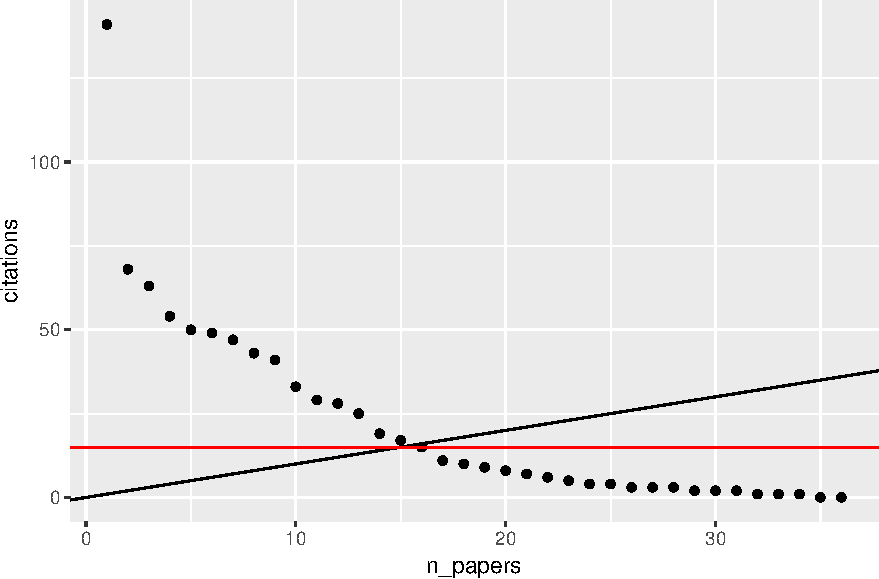
\includegraphics{muschelli_files/figure-latex/unnamed-chunk-13-1} \caption[Calculating an h-index]{Calculating an h-index.  Here we plot the number of papers versus the number of citations for that paper.  This plot is the basis for the h-index.  The X=Y line is displayed in black and the red line is where the curve passes the X=Y line, which is the h-index, a value of 15.}\label{fig:unnamed-chunk-13}
\end{figure}
\end{Schunk}

Additional indices can be created from the data, such as the
\emph{g}-index \citep{egghe2006theory}:

\begin{Schunk}
\begin{Sinput}
h_data = h_data %>% mutate(sum_citations = cumsum(citations))
g_index = max(which(h_data$sum_citations >= h_data$n_papers^2))
cat(paste0("Calculated g-index is ", g_index))
\end{Sinput}
\begin{Soutput}
Calculated g-index is 28
\end{Soutput}
\end{Schunk}

Overall, metrics based on citations and the year of publication can be
calculated, but longitudinal information is lacking. We will discuss
citation information over time in Section \ref{sec:citetime}.

\hypertarget{retrieving-information-about-an-author}{%
\subsection{Retrieving information about an
author}\label{retrieving-information-about-an-author}}

In \texttt{process\_author\_name}, we demonstrated how to get
information form an author with a relatively unique name. If this is not
the case, the \texttt{get\_complete\_author\_info}, which is the backend
function for \texttt{process\_author\_name}, can present more results.
In order to retrieve author IDs from first and last names, the
\texttt{get\_complete\_author\_info} can be used. Here we search for
authors with the last name West and first initial M:

\begin{Schunk}
\begin{Sinput}
last_name = "West"
first_name = "M"
auth_info_list = get_complete_author_info(last_name = last_name, first_name = first_name)
class(auth_info_list)
\end{Sinput}
\begin{Soutput}
[1] "list"
\end{Soutput}
\begin{Sinput}
names(auth_info_list)
\end{Sinput}
\begin{Soutput}
[1] "get_statement" "content"      
\end{Soutput}
\end{Schunk}

We see here, which is common in in some low-level functions returned
from the \texttt{rscopus} API, the output is a list with elements
\texttt{get\_statement}, which returns an object of class
\texttt{response} (from the \CRANpkg{httr} package \citep{httr}), and
\texttt{content}, which is the content from the response. Most times,
the \texttt{content} is of interest, but failed requrests may be
explored with the \texttt{get\_statement} output for debuggin.

Again, we can use \texttt{gen\_entries\_to\_df} convert that output into
a \texttt{data.frame}, which is more manageable:

\begin{Schunk}
\begin{Sinput}
coerced = gen_entries_to_df(auth_info_list$content$`search-results`$entry)
names(coerced)
\end{Sinput}
\begin{Soutput}
[1] "df"           "name-variant" "subject-area"
\end{Soutput}
\begin{Sinput}
head(coerced$df[, c("dc:identifier",  "preferred-name.surname",
                    "preferred-name.given-name", "affiliation-current.affiliation-name" )])
\end{Sinput}
\begin{Soutput}
          dc:identifier preferred-name.surname preferred-name.given-name
1 AUTHOR_ID:35480328200                   West                 Catharine
2 AUTHOR_ID:35419377800                   West                Malcolm J.
3  AUTHOR_ID:7003392768            Diener-West                     Marie
4  AUTHOR_ID:7402395730                   West                 Robert M.
5  AUTHOR_ID:7402068812                   West           Michael Abigail
6  AUTHOR_ID:7401998578                   West                  David M.
             affiliation-current.affiliation-name
1                        University of Manchester
2                James Cook University, Australia
3 Johns Hopkins Bloomberg School of Public Health
4                             University of Leeds
5         University of Pittsburgh Medical Center
6                               Massey University
\end{Soutput}
\end{Schunk}

We see this has information about the multiple authors returned, along
with names, variations on those names, number of documents, and
affiliations. We can then extract the author ID we want from this
\texttt{data.frame}. This process is wrapped in the
\texttt{get\_author\_info}:

\begin{Schunk}
\begin{Sinput}
auth_info_df = get_author_info(last_name = last_name, 
                              first_name = first_name)
head(auth_info_df)
\end{Sinput}
\begin{Soutput}
             auth_name       au_id          affil_id
1       Catharine West 35480328200          60003771
2      Malcolm J. West 35419377800          60019870
3    Marie Diener-West  7003392768          60006183
4       Robert M. West  7402395730          60012070
5 Michael Abigail West  7402068812 60012018 60023691
6        David M. West  7401998578          60008221
                                       affil_name
1                        University of Manchester
2                James Cook University, Australia
3 Johns Hopkins Bloomberg School of Public Health
4                             University of Leeds
5         University of Pittsburgh Medical Center
6                               Massey University
\end{Soutput}
\end{Schunk}

but we should note this information is condensed and a subset that is
available from \texttt{get\_complete\_author\_info}, also with more
standardized column names. Now, one could use the \texttt{au\_id}
retrieved from this output for searching.

If you had an affiliation ID, such as \texttt{60006183} for the Johns
Hopkins Bloomberg School of Public Health, we can pass this to
\texttt{get\_author\_info} or \texttt{process\_author\_name}:

\begin{Schunk}
\begin{Sinput}
spec_affil = get_author_info(
  last_name = last_name, 
  first_name = first_name,
  affil_id = 60006183)
spec_affil
\end{Sinput}
\begin{Soutput}
          auth_name      au_id affil_id
1 Marie Diener-West 7003392768 60006183
                                       affil_name
1 Johns Hopkins Bloomberg School of Public Health
\end{Soutput}
\end{Schunk}

Thus, we can use the combination of the names of the author and
affiliation information. This may be useful when searching multiple
authors at the same institution. We could also pass in
\texttt{affil\_name} instead of \texttt{affil\_id} to
\texttt{get\_author\_info}, but the name must be extremely specific for
institution as the function will call \texttt{get\_affiliation\_info},
which is discussed below.

\hypertarget{retrieving-information-about-multiple-authors}{%
\subsection{Retrieving information about multiple
authors}\label{retrieving-information-about-multiple-authors}}

In order to get information from multiple authors, one could loop over
author information, but this is inefficient for code and API calls. The
\texttt{complete\_multi\_author\_info} function can perform this
operation. One caveat is that it requires author identifiers and not
names. We can take the author IDs from \texttt{auth\_info\_df} to
retrieve information for all these authors:

\begin{Schunk}
\begin{Sinput}
all_author_info = complete_multi_author_info(au_id = auth_info_df$au_id)
names(all_author_info)
\end{Sinput}
\begin{Soutput}
[1] "get_statement" "content"       "au_id"        
\end{Soutput}
\end{Schunk}

This result is again a low-level output from the API. We can use the
\texttt{process\_complete\_multi\_author\_info} function to process this
into a more amenable solution:

\begin{Schunk}
\begin{Sinput}
processed = process_complete_multi_author_info(all_author_info)
head(names(processed))
\end{Sinput}
\begin{Soutput}
[1] "35480328200" "35419377800" "7003392768"  "7402395730"  "7402068812" 
[6] "7401998578" 
\end{Soutput}
\end{Schunk}

Now, each element is the author ID, which contains a list of
\texttt{data.frame}s. The \texttt{multi\_author\_info} will perform both
of these operations together. This result is still not ``tidy''
\citep{wickham2014tidy} in many respects, but parts can be combined
using \CRANpkg{purrr} \citep{purrr}:

\begin{Schunk}
\begin{Sinput}
journals = purrr:::map_df(processed, `$`, "journals", .id = "au_id")
head(journals)
\end{Sinput}
\begin{Soutput}
        au_id type                                        sourcetitle
1 35480328200    j                                     Cancer Letters
2 35480328200    j   Journal of Cancer Research and Clinical Oncology
3 35480328200    j                              Nature Reviews Cancer
4 35480328200    j Annals of the Royal College of Surgeons of England
5 35480328200    j                                     Cancer Letters
6 35480328200    j                         PLoS Computational Biology
           sourcetitle-abbrev     issn
1                Cancer Lett. 03043835
2 J. Cancer Res. Clin. Oncol. 01715216
3            Nat. Rev. Cancer 1474175X
4   Ann. R. Coll. Surg. Engl. 00358843
5                Cancer Lett. 18727980
6          PLoS Comput. Biol. 1553734X
\end{Soutput}
\end{Schunk}

Thus, in the above code we could compare the journals each author
published in compared to the other authors in the list.

\hypertarget{citations-over-time}{%
\subsection{Citations over time}\label{citations-over-time}}

\label{sec:citetime}

Some APIs from Elsevier are disabled by default (see
\url{https://dev.elsevier.com/api_key_settings.html}). Notably, the
Citations Overview API is disabled, which allows users to access
information about citations over time for articles of authors. This
information is particularly useful for creating bibliometric indices
that rely on subsetting data based on mininum or maximum year or
calculating time-dependent metrics. The \texttt{rscopus} package
interfaces with these APIs, but the API must be enabled for that
specific API key. On the Scopus website one can searching for authors,
select up to 15 authors, and then create a ``Citation Overview'', which
will give this citation information, which is in a CSV format. The
\pkg{rscopus} package provides a \texttt{read\_cto} function to read in
this data.

We also provide an example export from a single author in the package:

\begin{Schunk}
\begin{Sinput}
file = system.file("extdata", "CTOExport.csv", package = "rscopus")
citations_over_time = rscopus::read_cto(file)
names(citations_over_time)
\end{Sinput}
\begin{Soutput}
[1] "data"               "year_columns"       "author_information"
\end{Soutput}
\end{Schunk}

The real information is in the \texttt{data} element of this list, which
contains the yearly citation information (again titles have been
shortened):

\begin{Schunk}
\begin{Sinput}
yr_cols = citations_over_time$year_columns
citations_over_time = citations_over_time$data
citations_over_time = citations_over_time %>% 
  mutate(short_title = unique_title(`Document Title`))
head(citations_over_time[, c("short_title", yr_cols[1:5])])
\end{Sinput}
\begin{Soutput}
                            short_title <2008 2008 2009 2010 2011
1         Objective Evaluation Multiple     0    0    0    0    0
2              MIMoSA: Automated Method     0    0    0    0    0
3           Radiomic subtyping improves     0    0    0    0    0
4      Feasibility Coping Effectiveness     0    0    0    0    0
5     Freesurfer: Connecting Freesurfer     0    0    0    0    0
6 Thrombolytic removal intraventricular     0    0    0    0    0
\end{Soutput}
\end{Schunk}

In the citation overview, you must specify a range of years on Scopus,
with a maximum of 15 years. As many times this wide format is not what
you want to plot, or in a ``tidy'' format, the \pkg{rscopus} helper
function \texttt{read\_cto\_long} will read the data in long format,
done by \CRANpkg{tidyr} \citep{tidyr}. Here we use \pkg{dplyr} to
arrange the data by maximum number of citations per year:

\begin{Schunk}
\begin{Sinput}
long_cite = rscopus::read_cto_long(file)
long_cite = long_cite$data %>% 
  group_by(`Document Title`, year) %>% # get the citations per year
  summarize(citations = sum(citations), # aggregate - some duplicates merged
            `Publication Year` = unique(`Publication Year`)) %>% # keep the year in data
  mutate(short_title = unique_title(`Document Title`))
long_cite = long_cite %>% arrange(-citations, year, short_title)
head(long_cite[, c("short_title", "year", "citations")])
\end{Sinput}
\begin{Soutput}
# A tibble: 6 x 3
  short_title                           year  citations
  <chr>                                 <fct>     <int>
1 Minimally invasive surgery            2015         36
2 Minimally invasive surgery            2017         35
3 ISLES 2015 public                     2018         28
4 Large-scale radiomic profiling        2018         26
5 Thrombolytic removal intraventricular 2018         25
6 Minimally invasive surgery            2016         24
\end{Soutput}
\end{Schunk}

Thus, we have one record per year and article. Here we will plot the
cumulative citations per each paper over the years of publication and
label the top 3 cited papers:

\begin{Schunk}
\begin{Sinput}
# get cumulative sum
csum = long_cite %>% 
  # any missing data had no citations
  mutate(citations = ifelse(is.na(citations), 0, citations)) %>% 
  arrange(`Document Title`, year) %>% # sort for cumsum
  group_by(`Document Title`) %>% 
  mutate(citations = cumsum(citations))
# remove past and future with as.integer
csum = csum %>% 
  mutate(year = as.integer(as.character(year))) %>% 
  filter(!is.na(year)) %>% # remove < 2008 and > 2018 years
  filter(year >= `Publication Year` & citations > 0) # keep only relevant data for paper
# grab last citations and top 3 papers
last_year = csum %>% 
  arrange(`Document Title`, year) %>% # sort for slice later
  group_by(`Document Title`) %>% 
  slice(n()) %>% # keep last as max citations
  ungroup %>% arrange(-citations) %>% 
  head(3)  # get top 3
g = ggplot(csum, 
           aes(x = year, y = citations, color = short_title  )) +
  xlim(c(2010, 2018)) + geom_line() + 
  # label the titles numbers for top 3
  geom_text(data = last_year, size = 3, aes(label = short_title), 
            nudge_x = -1, nudge_y = 5)
# don't want label for document title - too many entries
g + guides(color = FALSE) + theme(text = element_text(size = 20))
\end{Sinput}

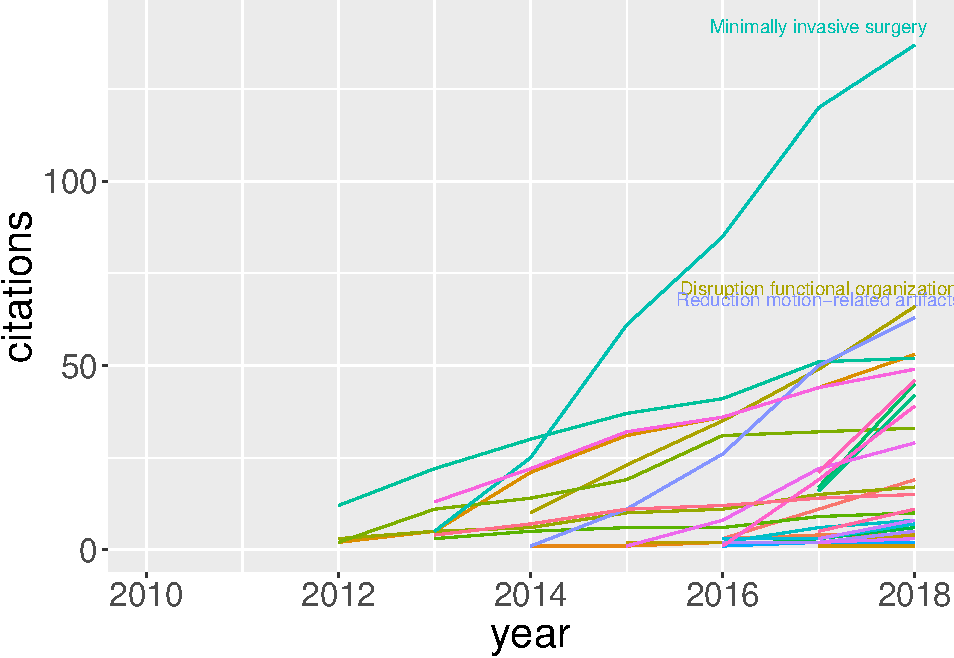
\includegraphics{muschelli_files/figure-latex/unnamed-chunk-24-1} \end{Schunk}

Thus, we can present visually how the number of citations has changed
and may be able to highlight which papers are gaining or waning in
citations over time. This plot may not provide deep insights, but the
same plot could be made by scientific sub-fields or for specific
journals, which may indicate trends in published articles for example.

\hypertarget{retrieving-affiliation-information}{%
\subsection{Retrieving affiliation
information}\label{retrieving-affiliation-information}}

In order to get information about an affiliation, the
\texttt{get\_affiliation\_info} can be used. Here we will look for the
pattern \texttt{Johns\ Hopkins}:

\begin{Schunk}
\begin{Sinput}
jhu_info = get_affiliation_info(affil_name = "Johns Hopkins")
head(jhu_info[, c("affil_id", "affil_name")])
\end{Sinput}
\begin{Soutput}
  affil_id                                              affil_name
1 60005248                                Johns Hopkins University
2 60001117                    The Johns Hopkins School of Medicine
3 60006183         Johns Hopkins Bloomberg School of Public Health
4 60001555                                  Johns Hopkins Hospital
5 60003443                      Johns Hopkins Medical Institutions
6 60022054 The Johns Hopkins University Applied Physics Laboratory
\end{Soutput}
\end{Schunk}

This function implicitly calls \texttt{affil\_search}, a lower-level
function which searches the affiliation information from Scopus.
Additional information can be extracted using \texttt{affil\_search},
but this typically includes a large number of records as it searches all
the documents. This affiliation ID again can be used to be more specific
when searching authors or documents.

\hypertarget{searching-articles-by-abstract}{%
\subsection{Searching articles by
abstract}\label{searching-articles-by-abstract}}

In some cases, one may have an article in mind and would like
information about the authors of that article In order to get the author
IDs from the article identifier, one can use the
\texttt{abstract\_retrieval} function. There are multiple identifiers
that can be used, such as PubMed ID, DOI, and we will use the Scopus ID
as that is what is returned from the \texttt{author\_data} output:

\begin{Schunk}
\begin{Sinput}
sc_id = jm$df$`dc:identifier`[1]
# retrieve abstract 
res = abstract_retrieval(id = sc_id, identifier = "scopus_id")
\end{Sinput}
\end{Schunk}

Here we will extract the abstract information from the result:

\begin{Schunk}
\begin{Sinput}
sc_info = res$content$`abstracts-retrieval-response`
substr(sc_info$coredata$`dc:description`, 1, 220)
\end{Sinput}
\begin{Soutput}
[1] "© 2018, The Author(s). We present a study of multiple sclerosis segmentation algorithms conducted at the international MICCAI 2016 challenge. This challenge was operated using a new open-science computing infrastructure."
\end{Soutput}
\end{Schunk}

Here we can extract information about the authors of the paper:

\begin{Schunk}
\begin{Sinput}
sc_df = purrr::map_df(sc_info$authors[[1]],
  as.data.frame, stringsAsFactors = FALSE, make.names = FALSE)
head(sc_df[, c("ce.given.name", "ce.initials", "X.auid")])
\end{Sinput}
\begin{Soutput}
  ce.given.name ce.initials      X.auid
1       Olivier          O.  8431704700
2        Audrey          A. 57203861434
3       Michaël          M. 57199507814
4      Baptiste          B. 57197801981
5       Florent          F. 57203867656
6       Mathieu          M. 57203864793
\end{Soutput}
\end{Schunk}

This information is located within the \texttt{author}
\texttt{data.frame} from the \texttt{full\_data} as well. Note, however
that the information from \texttt{author\_data} was obtained by
searching Scopus for an author, whereas the information from
\texttt{abstract\_retrieval} was obtained by searching for a specific
paper. As we took the first entry from the Scopus identifier, we will
subset the author data by \texttt{entry\_number} \texttt{1} from the
\texttt{author} \texttt{data.frame} to show the relevant info matches:

\begin{Schunk}
\begin{Sinput}
paper_author_info = jm$full_data$author
head(paper_author_info[paper_author_info$entry_number == 1, c("authid", "authname", "surname")])
\end{Sinput}
\begin{Soutput}
       authid     authname   surname
1  8431704700 Commowick O. Commowick
2 57203861434    Istace A.    Istace
3 57199507814      Kain M.      Kain
4 57197801981   Laurent B.   Laurent
5 57203867656     Leray F.     Leray
6 57203864793     Simon M.     Simon
\end{Soutput}
\end{Schunk}

Thus, if we retrieve a single author's information, we can gather other
author IDs from this directly. If we have a specific paper, we can
retrieve author IDs from that paper information as well.

\hypertarget{object-retrieval}{%
\subsection{Object retrieval}\label{object-retrieval}}

Along with metadata, abstract, and other information about a paper,
additional objects may be accessed, such as figures, movies, or
supplemental material The \texttt{object\_retrieval} function will
return the objects associated with the identifier. The
\texttt{process\_object\_retrieval} will convert the output into a tidy
\texttt{data.frame}:

\begin{Schunk}
\begin{Sinput}
objects = object_retrieval("S1053811915002700", identifier = "pii", verbose = FALSE)
obj_df = process_object_retrieval(objects)
head(obj_df[, c("type", "url", "mime_type")])
\end{Sinput}
\begin{Soutput}
             type
1 IMAGE-THUMBNAIL
2 IMAGE-THUMBNAIL
3 IMAGE-THUMBNAIL
4 IMAGE-THUMBNAIL
5 IMAGE-THUMBNAIL
6 IMAGE-THUMBNAIL
                                                                                                url
1 https://api.elsevier.com/content/object/eid/1-s2.0-S1053811915002700-gr1.sml?httpAccept=image/gif
2 https://api.elsevier.com/content/object/eid/1-s2.0-S1053811915002700-gr2.sml?httpAccept=image/gif
3 https://api.elsevier.com/content/object/eid/1-s2.0-S1053811915002700-gr3.sml?httpAccept=image/gif
4 https://api.elsevier.com/content/object/eid/1-s2.0-S1053811915002700-gr4.sml?httpAccept=image/gif
5 https://api.elsevier.com/content/object/eid/1-s2.0-S1053811915002700-gr5.sml?httpAccept=image/gif
6 https://api.elsevier.com/content/object/eid/1-s2.0-S1053811915002700-gr6.sml?httpAccept=image/gif
  mime_type
1 image/gif
2 image/gif
3 image/gif
4 image/gif
5 image/gif
6 image/gif
\end{Soutput}
\end{Schunk}

where the URL provides the link to download the object. Here we will
subset the output to high-resolution images, and pass the URL for the
first to the \texttt{download\_object} function. This will return the
content of the image, as well as download the image to disk (with path
\texttt{outfile}):

\begin{Schunk}
\begin{Sinput}
obj_df = obj_df[ grepl("image/jpeg", obj_df$mime_type),]
obj_df = obj_df[ obj_df$type %in% "IMAGE-HIGH-RES",]
object = download_object(obj_df$url[1])
object$outfile
\end{Sinput}
\begin{Soutput}
[1] "/var/folders/1s/wrtqcpxn685_zk570bnx9_rr0000gr/T//Rtmpmfe411/file18415a23ca8a.jpg"
\end{Soutput}
\end{Schunk}

One can then view the output using the system viewer using
\texttt{utils::browseURL}. The \texttt{download\_objects} function is a
convenience wrapper for \texttt{lapply(url,\ download\_object)} when
passing in all the URLs from the output of \texttt{object\_retrieval}.

\hypertarget{conclusion}{%
\section{Conclusion}\label{conclusion}}

The \pkg{rscopus} package provides an interface to the Scopus API
through R. The package allows users to retrieve information about
authors, individual articles, or institutions from the API. The
information that can be obtained is limited by the scopes enabled by the
API key through Elsevier and the associated organization. We have shown
how to obtain an API key and specific use cases, which we believe covers
the a number of the needs of the users.

More advanced usage requires additional information about the Scopus API
and its querying specifications. The future direction of this package is
to create helper functions to construct queries for more targeted views
of the data. Additional APIs from Elsevier have functions for access,
such as SciDirect with the \texttt{rscopus::sciencedirect\_search}
function, but the main focus of the package has been Scopus. Although
the goal is to keep all functionality up to date with the number of
APIs, the main focus will be consistency and stability with respect to
Scopus. All the code and figures used to create this paper are located
at \url{https://github.com/muschellij2/scopus} and the paper was created
using the \CRANpkg{rticles} package \citep{rticles}.

\hypertarget{supplemental-material}{%
\section{Supplemental Material}\label{supplemental-material}}

Here is the simple parser \texttt{unique\_title} to find the first 3
relevant words of the title after removing non-relevant words froma list
in the \CRANpkg{stopwords} package \citep{stopwords}:

\begin{Schunk}
\begin{Sinput}
unique_title = function(x) {
  ss = sapply(strsplit(x, split = " "), 
              function(x) {
                x = x[ !tolower(x) %in% stopwords::stopwords()]
                x = x[ !x %in% c("-", "?", "--", 1:100)]
                paste(x[1:3], collapse = " ")
              })
  stopifnot(length(unique(ss)) == length(unique(x)))
  ss
}
\end{Sinput}
\end{Schunk}

\bibliography{muschelli.bib}

\address{%
John Muschelli\\
Department of Biostatistics, Johns Hopkins Bloomberg School of Public
Health\\
615 N Wolfe St Baltimore, MD 21205\\
}
\href{mailto:jmuschel@jhsph.edu}{\nolinkurl{jmuschel@jhsph.edu}}

